\documentclass[11pt]{article}
\usepackage[margin=1in]{geometry}
\usepackage{graphicx}
\usepackage{hyperref}
\usepackage{natbib}
\bibliographystyle{apalike}
\title{The Diffusion State: AI Pilot Zones, Smart Factories, and the Hub Architecture of China’s Industrial AI Adoption}
\author{Research draft --- \texttt{paper/draft\_v1\_submission.md}}
\date{\today}
\begin{document}
\maketitle
\begin{abstract}
See \texttt{paper/draft\_v1\_submission.md} for full text (Pass 1--6 + appendix).
\end{abstract}
\section*{Note}
Import \texttt{paper/draft\_v1\_submission.md} via Pandoc or paste section text here.
\begin{figure}[ht]
  \centering
  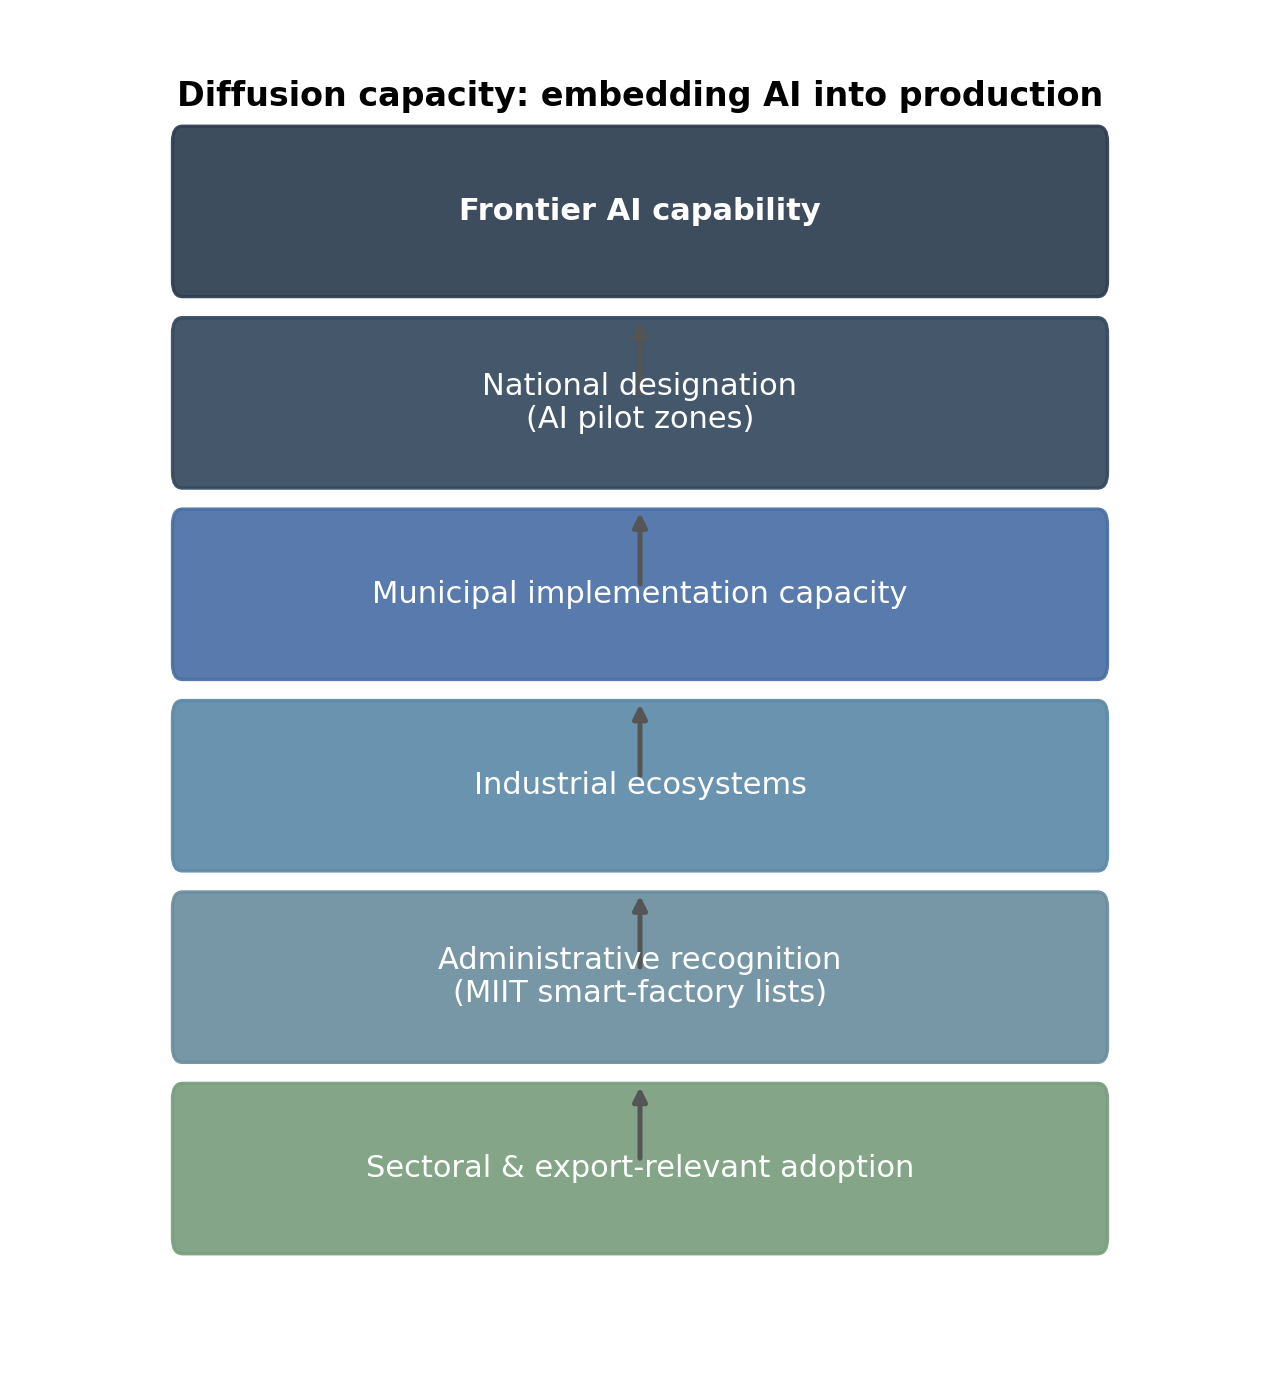
\includegraphics[width=0.92\linewidth]{figures/fig_1_diffusion_state_architecture.png}
  \caption{Conceptual architecture: from frontier AI capability to sectoral and export-relevant industrial adoption.}
\end{figure}
\begin{figure}[ht]
  \centering
  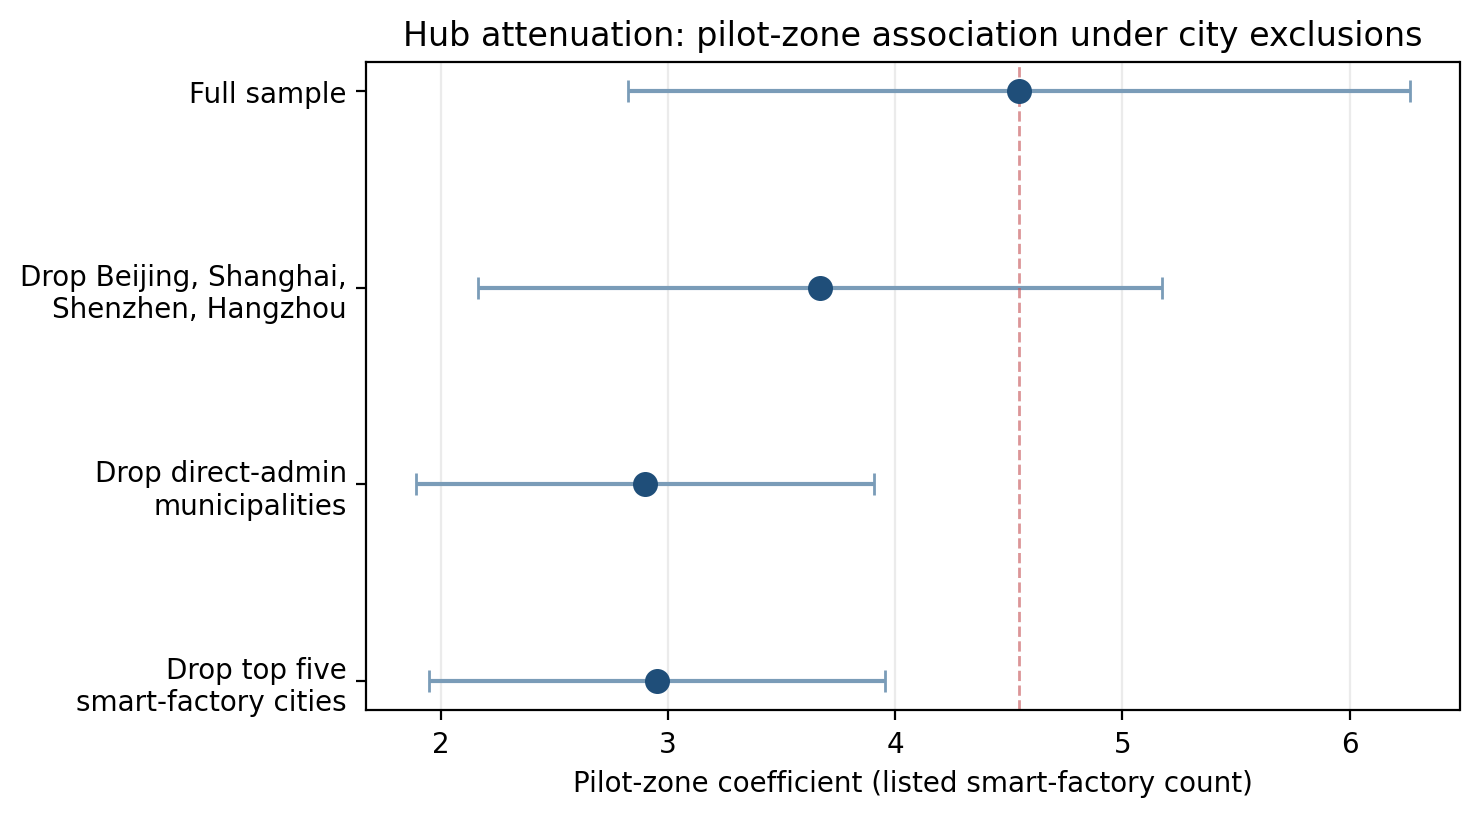
\includegraphics[width=0.92\linewidth]{figures/fig_2_hub_attenuation_pilot_coefficients.png}
  \caption{Pilot-zone coefficient on listed smart-factory counts under hub-exclusion rules (95% CI).}
\end{figure}
\begin{figure}[ht]
  \centering
  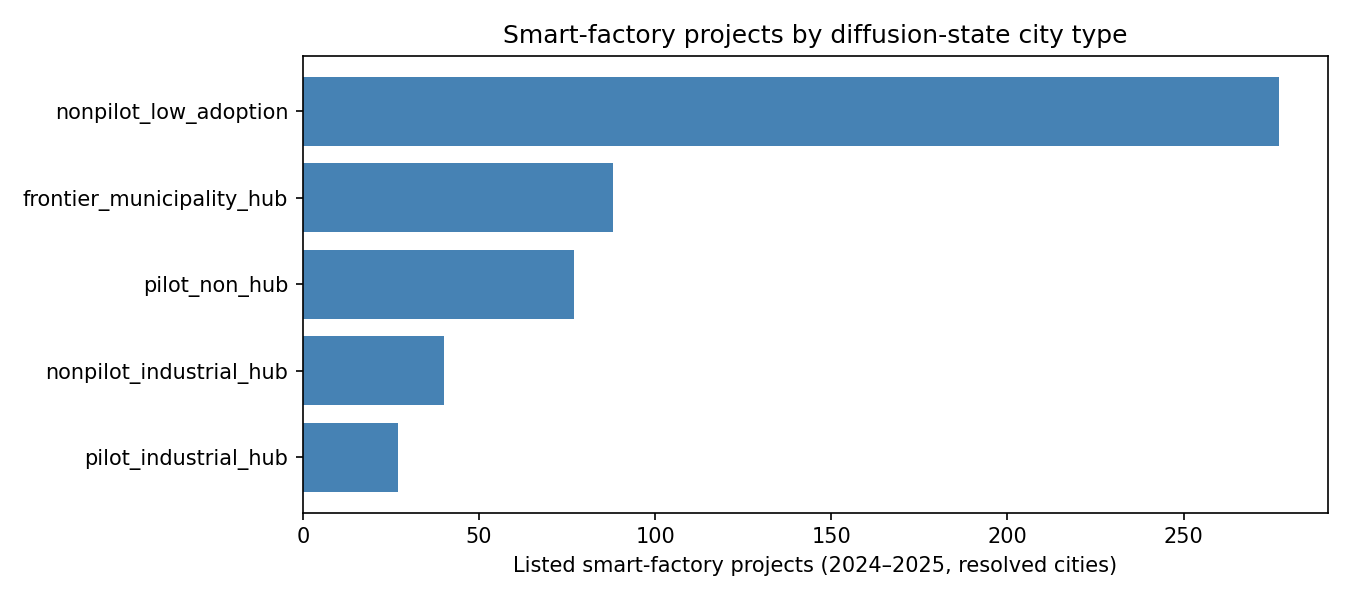
\includegraphics[width=0.92\linewidth]{figures/fig_3_city_typology_smart_factory_counts.png}
  \caption{Listed smart-factory projects by ex ante diffusion-state city type (2024–2025, resolved cities).}
\end{figure}
\bibliography{references}
\end{document}
